\documentclass[a4paper]{article}
\usepackage[utf8]{inputenc}
\usepackage[T1,T2A]{fontenc}
\usepackage[russian]{babel}
\usepackage{amsmath}
\usepackage{amsfonts}
\usepackage{amssymb}
\usepackage{mathtools,bm,etoolbox}
\usepackage{indentfirst}
\usepackage{hyperref}
\usepackage{xcolor}
\usepackage{listings}
\usepackage{graphicx}
\usepackage{float}
\graphicspath{ {/home/maxim/study/my_project/linear_classifiers/notebooks/} }

\newcommand{\ik}{I(\wk)}
\newcommand{\w}{\bm{w}}
\newcommand{\wk}{\bm{w_k}}
\newcommand{\xj}{\bm{x_j}}
\newcommand{\yk}{y_k}
\newcommand{\xk}{\bm{x_k}}
\newcommand{\xkj}{x_{kj}}
\newcommand{\W}{\bm{W}}
\newcommand{\veps}{\bm{\varepsilon}}
\newcommand{\E}{\mathbb{E}}

\definecolor{dkgreen}{rgb}{0,0.6,0}
\definecolor{gray}{rgb}{0.5,0.5,0.5}
\definecolor{mauve}{rgb}{0.69,0.43,0.16}

\righthyphenmin=2
\tolerance=360

\lstset{frame=tb,
  language=Python,
  aboveskip=3mm,
  belowskip=3mm,
  showstringspaces=false,
  columns=flexible,
  basicstyle={\small\ttfamily},
  numbers=none,
  numberstyle=\tiny\color{dkgreen},
  keywordstyle=\color{dkgreen},
  commentstyle=\color{gray},
  stringstyle=\color{mauve},
  breaklines=true,
  breakatwhitespace=true,
  tabsize=3
}
\hypersetup{%
  colorlinks=true,% hyperlinks will be coloured
  linkcolor=blue,% hyperlink text will be green
  linkbordercolor=blue,% hyperlink border will be red
}

\author{Maxim Zmeev}
\title{Сравнительный анализ линейных классификаторов}
\begin{document}
\begin{titlepage}
\centering
\par\vspace{1cm}{\scshape\Large Московский физико-технический институт(Государственный университет) \par}

\vspace{1cm}{\scshape\Large Факультет управления и прикладной математики\par}

\vspace{1.5cm}{\huge\bfseries Сравнительный анализ линейных классификаторов \par}

\vfill

\vspace{1.5cm}{\bfseries Выпускная квалификационная работа на степень бакалавра студента 376 группы Змеева Максима Владимировича \par}

\vfill

\par\vspace{1cm}{\scshape\Large Научный руководитель: профессор Рязанов В.В. \par}

\end{titlepage}

\newpage

\tableofcontents

\newpage

\section{Введение}

В наше время машинное обучение завоевало строго положительную репутацию. В данных часто есть закономерности, которые не удаётся отследить невооруженным глазом. Для этого существует много математических моделей, которые находят зависимости между данными и позволяют делать предсказания. Предсказательные модели можно использовать практически в любой сфере. Самые простые предсказания строятся на основе линейных моделей, которые отличаются от других высокой скоростью обучения, но меньшей предсказательной силой. В данной работе рассмотрены основные известные виды линейных классификаторов, к ним добавлены два менее известных подхода(релаксационный метод и метод сведения к линейному программированию). Оба подхода решают задачу поиска максимальной совместной подсистемы системы линейных неравенств. Представляет интерес сравнить их между собой и с уже проявившими себя методами. Каждый классификатор реализован в Python3 с максимальным использованием библиотеки numpy для ускорения вычислений. Все классификаторы сравнивались как на модельных данных, так и на настоящих данных, взятых из известных датасетов. Сравнение производилось по доле правильных ответов(классы всегда достаточно сбалансированы поэтому эта метрика вполне подходит). Также сравнивались времена работы классификаторов. Было выяснено, что сведение к линейному программированию имеет то преимущество, что позволяет сказать, можно ли с самого начала построить разделяющую гиперплоскость между объектами разных классов. Релаксационный метод проявил себя как самый быстро обучающийся, а три оставшиеся в очередной раз подтвердили свою высокую скорость и хорошую для линейной классификации точность предсказаний.

\section{Постановка задачи}

\subsection{Для двух классов}
Есть N элементов, каждый из которых принадлежит одному из двух классов. Каждый объект представляет из себя вектор размерности D.  Для $N_{train}$ элементов их классы известны: 
$$\yk = \begin{cases}
1, & \text{если объект } \xk \text{ принадлежит классу 1}\\
0, & \text{если объект } \xk \text{ принадлежит классу 0}
\end{cases}.
$$Для остальных $N_{test} = N - N_{train}$ элементов(тестовой выборки) их классы нужно предсказать для тестовых $N_{test}$ объектов.

\subsection{Для любого числа классов}

Имеется $N$ объектов, каждый из которых принадлежит одному из $M$ классов. Каждый объект имеет $D$ числовых признаков. Для $N_{train}$ объектов(обучающей выборки) их классы известны. 
$$\yk = \begin{cases}
0, & \text{если объект } \xk \text{ принадлежит классу 0}\\
1, & \text{если объект } \xk \text{ принадлежит классу 1}\\
...\\
M, & \text{если объект } \xk \text{ принадлежит классу M}\\
\end{cases}.
$$
Для остальных $N_{test} = N - N_{train}$ элементов(тестовой выборки) их классы нужно предсказать для тестовых $N_{test}$ объектов.

\section{Предлагаемые методы решения}

\subsection{Для двух классов}

\subsubsection{Релаксационный метод}

Предлагается пытаться отделять объекты классов друг от друга гиперплоскосью в D-мерном пространстве. Гиперплоскость задаётся (D+1) -мерным вектором $\w$. Объект $\xk$ считается объектом класса 1, если $w_{0} + \sum_{j = 1}^{D}x_{ij} \cdot w_j > 0$ и объектом класса 0, если $w_{0} + \sum_{j = 1}^{D}x_{ij} \cdot w_j < 0$(вероятность, что непрерывно распределенная случайная величина будет равна ровно нулю в такой линейной комбинации, равна нулю, поэтому качество не будет ухудшено вне зависимости от того, будет ли присваиваться нулевой или первый класс объектам, на которых оба неравенства не выполнятся). Все векторы $\xk$ для удобства преобразуются в (D+1)-мерные вектора вида $(1, x_{k1}, x_{k2}, .., x_{kD})$, чтобы можно было более кратко писать $\xk^{T}\w$. Для нахождения верктора $\w$ минимизируется функционал:
\begin{equation} \label{01}
L = \frac{1}{N_{train}} \sum_{k = 1}^{N_{train}}([\xk^{T}\w >= 0] \cdot (1 - y_k) + [\xk^{T}\w < 0] \cdot y_k)
\end{equation}
То есть долю ошибок при классификации обучающей выборки.

Составляется система неравенств: 

\begin{equation}\label{02}
\begin{cases}
\xk^T\w \cdot (-1) ^ {\yk} >=0, & k = \overline{1,N_{train}} 
\end{cases}
\end{equation}

Теперь получается, что нужно найти такой вектор $w$, чтобы максимальное число неравенств из (\ref{02}) выполнялось. Задача сводится к поиску максимальной совместной подсистемы системы неравенств.

Далее под $\xk$ подразумевается $\xk \cdot (-1)^{y_k}$ как коэффициент одного уравнения системы (\ref{02}). Допустим, система совместна. Искать её решение предлагается, строя последовательность $\bm{w_1}, \bm{w_2} ... \wk ...$. Введено обозначение $I(\wk) = \{k|\xk^T\w < 0\}$. Далее идут разные варианты построения последовательности $\{\wk\}_{k = 1}^{K}$, а точнее выбор направления $\bm{d_w}$ в $\bm{w_{k + 1}} = \wk + \theta_{k+1} \cdot \bm{d_w}$:
\begin{itemize}

\item
\begin{equation}
\bm{d_w} = \bm{x_q} \cdot \frac{\bm{x_q}^T\wk}{||\bm{x_q}||^2}, \text{ где } q = \arg\underset{j \in \ik}{\max} |\xj^T\wk|
\end{equation}

\item
\begin{equation} \label{04}
\bm{d_w} = \bm{z} \cdot \frac{\sum_{j \in \ik} (\xj^T\wk)^2 }{||\bm{z}||^2}, \text{ где } \bm{z} = \sum_{j \in \ik}\xj \cdot |\xj^T\wk|
\end{equation}

\item
\begin{equation}
\bm{d_w} = \bm{z} \cdot \frac{\sum_{j \in \ik} \lambda_j \cdot |\xj^T\wk| }{||\bm{z}||^2}, \text{ где }  \bm{z} = \sum_{j \in \ik} \xj \cdot \lambda_j; \lambda_j \ge 0
\end{equation}
$\lambda_j$ находятся как решения задачи максимизации числа неравенств, которые сменяют свой знак с отрицательного на положительный.
\end{itemize}

Для таких случаев при $0 \le \theta \le 2$ и, если система совместна, доказано\cite{agmon}:
$$
\rho(\bm{w_{k+1}}, Q) \le \sigma \cdot \rho(\bm{w_{k}}, Q), 0 < \sigma < 1 
, \text{гдe }Q \text{ - множество решений}
$$

Вернёмся к случаю, когда система не обязательно совместна. Ясно, что тогда не будет найдено решение полной системы, потому что не абсолютно любые объекты отделяются гиперплоскостью, также всегда можно встретить выбросы. То есть нужно отбрасывать некоторые из неравенств. Предлагается это делать через каждые несколько итераций, отбрасывая те неравенства, которые чаще всего не выполняются. Таким образом, наступит момент, когда система станет совместна, и решение будет найдено.

Для увеличения скорости сходимости рекомендуется решать систему:
\begin{equation}
\begin{cases}
\xk^T\w \cdot (-1) ^ {\yk} >= \varepsilon, & k = \overline{1,N_{train}} 
\end{cases}
\end{equation}

Итак, данный классификатор, имеет 3 гиперпараметра: 
\begin{itemize}
\item $\varepsilon$ - поправка к неравенствам;
\item $k$ - число шагов, после которого отбрасываются неравенства, которые чаще всего не выполнялись;
\item $\theta$ - скорость обучения.
\end{itemize}

Данное число, конечно, можно расширить засчёт того, что скорость обучения можно менять по мере приближения к множеству решений, одновременно с этим можно менять и число шагов, которое делается до отбрасывания неравенств по мере обучения.

\subsubsection{Сведение к линейному программированию}

Задача снова сводится к поиску максимальной совместной подсистемы системы линейных неравенств. Снова те неравенства, чьи объекты принадлежат к классу 0, умножаются на -1. Введится дополнительная переменная $\varepsilon$, которую нужно максимизировать в следующей задаче:
\begin{equation}
\begin{cases}
\varepsilon \rightarrow \max \\
\xk^T\w \cdot (-1)^{y_k} > \varepsilon, & k = \overline{1, N_{train}}
\end{cases}
\end{equation}

Если система несовместна, то очевидно, что решение будет $\varepsilon = \epsilon \le 0$. Далее предлагается отбрасывать неравенства. Отбрасывается то, для которого достигается максимум величины $$\frac{\frac{1}{|I_0|} \cdot (\underset{i \neq j}{\underset{i \in I_0}{\sum}}w_i^T)w_j}{||\underset{i \neq j}{\underset{i \in I_0}{\sum}}w_i||\cdot ||w_j|| }$$

Такая процедура выполняется, пока $\varepsilon$ не станет больше нуля.

Итак, получили классификатор с 2 гиперпараметрами:
\begin{itemize}
\item $k$ - число шагов, после которого мы отбрасываем неравенства, самые отклюняющиеся от остальных невыполненных;
\item $part\_to\_exclude$ - доля неравенств, которую мы будем исключать из системы.
\end{itemize}

\subsubsection{Логистическая регрессия}

Теперь хочется ускорить процесс обучения. Для этого нужно сделать функцию потерь $L$ непрерывно дифференцируемой. Хорошо подходит сигмоида:
\begin{equation} \label{sigmoid}
\sigma(\xk) = \frac{1}{1 + \exp^{ - \xk^T\w \cdot (-1)^{\yk}}}
\end{equation}
Если объект k классифицировали как объект класса 1, то значение $\xk^T\w > 0$. Если решение принято верно(true positive), то степень экспоненты будет положительной, значит вся дробь будет стремиться к нулю при увеличении значения $\xk^T\w$. Если решение ошибочное(false positive), то степень экспоненты будет отрицательной, а значит вся дровь будет стремиться к единице при отдалении $\xk^T\w$ от единицы вправо. Аналогично, если $\xk^T\w < 0$ и выбор правильный(true negative), то вся дробь будет тем ближе к нулю, чем левее от нуля значение $\xk^T\w$, если выбор неправильный(false negative), то вся дробь будет тем ближе к единице, чем больше значение $\xk^T\w$. То есть при правильных ответах значение (\ref{sigmoid}) близко к единице, при неправильных - к нулю.

Функция потерь - это сумма таких сигмоид для каждого объекта из обучающей выборки:
\begin{equation}
\bm{L} = \sum_{k = 1}^{N_{train}}\sigma(\xk)
\end{equation}

Подсчёт градиента сигмоиды: 
\begin{multline*}
\frac{\partial \sigma(\xk)}{\partial w_j} = \\ = - \frac{1}{(1 + \exp(-\xk^T\w(-1)^{\yk}))^2} \cdot \exp(-\xk^T\w(-1)^{\yk}) \cdot (-\xkj\cdot(-1)^{\yk})=  \\ =
\frac{1}{1 + \exp(-\xk^T\w(-1)^{\yk})} \cdot \frac{\exp(-\xk^T\w(-1)^{\yk})}{1 + \exp(-\xk^T\w(-1)^{\yk})} \cdot (-1)^{\yk + 1} \cdot \xkj = \\ =
\sigma(\xk^T\w) \cdot (1 - \sigma(\xk^T\w)) \cdot \xkj \cdot (-1)^{\yk + 1} \text{, при } k = \overline{1, N_{train}}, j = \overline{1, D + 1}
\end{multline*}

Видно, что градиент сигмоиды легко выражается через саму сигмоиду, здесь же нужно добавить производную показателя сигмоиды.

Итак, эту функцию потерь минимизируют итерационным методом, использующим аналитический подсчёт градиента, например, градиентным спуском и тем самым находят решение.

\subsection{Для любого числа классов}

\subsubsection{Метод опорных векторов (SVM)}

Теперь имеется более, чем два класса, поэтому бля принятия решения недостаточно одной разделяющей гиперплоскости. Для каждого класса заводится свой вектор весов $\wk, k = \overline{1, M}$. В итоге имеется матрица весов $\W = ||\bm{w_1}, \bm{w_2}, ..., \bm{w_M}||$. Для определения класса объекта $\bm{x}$ вычисляется произведение $\W^T\bm{x}$ - вектор оценок. Выбирается тот класс, чья оценка самая высокая.

Функция потерь $L_i$ на одном объекте выглядит следующим образом:
\begin{equation}
\bm{L_k} = \sum_{j \neq y_k}\max{(0, \xk^T\wk - \xk^T\bm{w_{y_k}} + \Delta)}
\end{equation}

Также есть смысл использовать регуляризацию 
\begin{equation}
R(W) = \sum_{i = 1}^{D}\sum_{j = 1}^M W_{i,j}^2
\end{equation}

Итоговая функция потерь может быть записана как
\begin{equation*}
\bm{L} = \frac{1}{N}\sum_{i = 1}^N L_i + \lambda R(W)
\end{equation*}

Или более полно:
\begin{equation}
L = \frac{1}{N}\sum_{k = 1}^N\sum_{j \neq y_k}\max{(0, \xk^T\wk - \xk^T\bm{w_{y_k}} + \Delta)}  + \lambda\sum_i\sum_j W_{i,j}^2
\end{equation}

Остаётся найти минимум по весам данной функции. Оптимизация проводится градиентным спуском. Производная функции потерь по весу верного класса выражается в виде:
\begin{equation}
\nabla_{\bm{w_{y_k}}} L_k = -\left(\sum_{j \neq y_k} \bm{1}(\xk^T\bm{w_j} - \xk^T\bm{w_{y_k}} + \Delta > 0)\right) \xk
\end{equation}
где $\bm{1}$ - функция-индикатор, равная единице, если условие верно, и нулю, если условие не верно.
По остальным весам ($j \neq y_k$):
\begin{equation}
\nabla_{\bm{w_j}} L_k = \bm{1}(\xk^T\bm{w_j} - \xk^T\bm{w_{y_k}} + \Delta > 0) \xk
\end{equation}

Данный классификатор имеет 2 гиперпараметра:
\begin{enumerate}
\item $\Delta$ - сдвиг в функции потерь;
\item $\lambda$ - коэффициент перед весами. Чем он больше, тем сильнее регуляризируются веса.
\end{enumerate}

\subsubsection{Минимизация кросс-энтропии (Softmax)}

Пусть имеется некая оценочкая функция $f_j(\xk, \W)$, в данном случае $f_j(\xk, \W) = \W^T\xk$, дающая оценку принадлежности объекта $\xk$ классу j. Функция потерь в таком случае выглядит следующим образом:
\begin{equation}
L_k = - \log\left(\frac{e^{f_{y_k}(\xk, \W)}}{\sum_je^{f_j(\xk, \W)}}\right) = 
- f_{y_k} + \log\sum_je^{f_j(\xk, \W)}
\end{equation}
Кросс-энтропия между оценённым распределением $q$ и настоящим $p$ даётся формулой:
\begin{equation}
H(p, q) = - \sum_x p(x)\log q(x)
\end{equation}

В нашем случае $q = \frac{e^{\bm{f_{y_k}(\xk, \W)}}}{\sum_je^{\bm{f_j(\xk, \W)}}}$, $p = (0,0,0,..., 1, ..., 0)$, где единице стоит на $y_k$ месте. То есть данная функция потерь минимизирует кросс-энтропию между оценённым и истинным распределением.

Также такой выбор функции потерь можно интерпретировать как желание найти максимум логарифма функции правдоподобия для данного рапределения.

Итоговая функция потерь выглядит следующим образом:
\begin{equation}
L = \frac{1}{N}\sum_k \W^T\xk + R(W)
\end{equation}

\paragraph*{Практический совет:} из-за использования экспонент в функции потерь могут возникнуть проблемы с численными подсчётами, потому что значения $e^{f_j(\xk, \W)}$ могут оказаться очень большими. Для избежания этих проблем стоит сделать поправку на константу:
\begin{equation}
\frac{e^{f_{y_k}(\xk, \W)}}{\sum_je^{f_j(\xk, \W)}} = \frac{Ce^{f_{y_k}(\xk, \W)}}{C\sum_je^{f_j(\xk, \W)}} = \frac{e^{f_{y_k}(\xk, \W) + \log C}}{\sum_je^{f_j(\xk, \W) + \log C}}
\end{equation}

Для уверенности можно выбрать $\log(C) = - \max_jf_j$. Тогда все экспоненты будут давать значение меньше единицы, что даст уверенность в точности вычислений.

Остаётся подсчитать градиент функции потерь:
\begin{align*}
p_k &= \frac{e^{f_{y_k}}}{\sum_je^{f_j}}     &       L_k &= -\log p_k
\end{align*}

\begin{eqnarray}
\frac{\partial L_k}{\partial f_j} = p_j - \bm{1}(k = y_k) \\
\frac{\partial L_k}{\partial \bm{w_j}} = \left(p_j - \bm{1}(k = y_k)\right) \xk
\end{eqnarray}

\section{Реализация методов}

\subsection{Релаксационнный метод}

Везде далее np - библиотека numpy, ускоряющая и упрощающая многие вычисления. Итак, приступим к реализации: создаётся свой класс, который называется \textbf{one\_weight\_linear\_model}, имеющий вектор весов $w$, число объектов \textbf{N}, число признаков \textbf{D}(включая константу), число шагов перед исключением неравенств \textbf{steps\_to\_exclude}, параметр $\theta$, который называется \textbf{theta}, параметр $\varepsilon$ : \textbf{eps} и долю исключающихся неравенств \textbf{part\_to\_exclude}, потому что, если исключать по одному неравенству на большом наборе данных, то слишом долго будет находиться решение. Вектор весов сначала пустой, так как размерность данных изначально неизвестна.
\begin{lstlisting}
class one_weight_linear_model():
	def __init()__(self, method, theta, eps, steps_to_exclude, part_to_exclude):
		self.w = None
		self.D = None
		self.N = None
		self.theta = theta
		self.eps = eps
		self.part_to_exclude = part_to_exclude
		self.steps_to_exclude = steps_to_exclude
\end{lstlisting}

Далее нужно описать метод \textbf{fit(self, X, y)}, принимающий на вход матрицу объектов и вектор номеров классов. Но для начала преобразовывается \textbf{X} так, что для объектов класса 0 добавляется ещё один константный признак, равный единице, а объекты класса 1 также получают константный признак, а затем домножаются на -1. Таким образом матрица X - матрица коэффициентов системы линейных неравенств, для которой все неравенства должны быть больше нуля. Так же инициализируются веса модели \textbf{w}. Воспользовавшись простыми соображениями о том, что примерно половина весов будет больше нуля, половина - меньше нуля, \textbf{w} инициализируются случайными числами из нормального распределения. Чтобы отклик не был слишком большим, для большего числа размерности устанавливается меньшая дисперсия, пропорционально $\sqrt{k}$. Эти подготовительные действия помещаются в отдельный метод \textbf{prepare\_data(self, X, y)}
\begin{lstlisting}
def prepare_data(self, X, y):
	X = np.array(X)
	self.N = X.shape[0]
	X = np.concatenate((X, np.ones([self.N, 1])), axis=1)
	self.D = X.shape[1]
	self.w = np.random.normal(0, 2. / self.D, self.D)
	X = np.apply_along_axis(lambda a: a * (-1) ** (y + 1), 0, X)
	return X
\end{lstlisting}

Вызов этого метода делается первым в методе \textbf{fit}. Далее нужно приготовить словарь номеров неравенств, которые не выполняются. Для этого предлагается хранить вектор \textbf{unfulfilled}(изначально из нулей) размера n. Если неравенство под номером i не было выполнено, то i-тый элемент вектора \textbf{unfulfilled} под номером i будет увеличен на единицу. Теперь нужно выбрать, какой шаг будет делаться. Здесь реализован второй вариант. Написана функция \textbf{calc\_dw(self, X)}, которая будет высчитывать направление шага, которое будет умножаться на \textbf{theta}:
\begin{lstlisting}
def calc_dw(self, X):
	negatives = X[X.dot(self.w) <= 0]
	scalar_mults = np.abs(negatives.dot(self.w))
	dw = np.sum(np.apply_along_axis(lambda a: a * scalar_mults, 0, negatives), axis=0)
 	dw *= np.sum(scalar_mults ** 2) / np.sum(dw ** 2)
 	return dw
\end{lstlisting}

Здесь \textbf{negatives} - те объекты, для которых неравенства не выполняются, \textbf{scalar\_mults} - это матрица попарных произведений $\bm{x_{ji}w_{ki}}$, где j - номер объекта, i - номер признака.

Есть один ньюанс: может случиться так, что dw окажется очень маленьким по норме. для таких случаев написано дополнительное условие, которое бы не позволяло делить на 0 в вычислении согласно формуле (\ref{04}):
\begin{lstlisting}
if np.any(np.abs(dw) > 1e-10):
	dw *= np.sum(scalar_mults ** 2) / np.sum(dw ** 2)
else:
	dw *= np.sum(scalar_mults ** 2) / 1e-11
\end{lstlisting}
Здесь, если видно, что по модулю \textbf{dw} очень мало, то делится не на 0, а на очень маленькую величину.

Теперь для обучения нужно отбрасывать те неравенства, которые не выполняются чаще всего. Для этого пишется метод \textbf{delete\_worst(self, X, unfulfilled)}, который на вход получает \textbf{X}  - матрицу объекты-призна\-ки и вектор \textbf{unfulfilled}, содержащий в себе частоту невыполнения каждого из неравенств:
\begin{lstlisting}
def delete_worst(self, X, unfulfilled):
	for i in range(max(1, int(self.N * self.part_to_exclude))):
		num_to_del = np.argmax(unfulfilled)
		X = np.delete(X, num_to_del, 0)
		unfulfilled = np.delete(unfulfilled, num_to_del, 0)
	return X, unfulfilled
\end{lstlisting}

Видно, что исключается по крайней мере одно неравенство, которое чаще всего не выполняется.

Итак, всё готово для написания метода \textbf{fit}. Последовательность действий довольно проста: подготавливается матрица объекты-признаки методом \textbf{prepare\_data}, затем идёт цикл, где на каждом шаге делается один шаг на \textbf{dw}. Каждые \textbf{steps\_to\_exclude} шагов отбрасывается одно или часть \textbf{part\_to\_exclude} неравенств, пока не будут выполнены все неравенства оставшейся системы.
\begin{lstlisting}
def fit_relax(self, X, y):
	if self.method == 'relax':
		X = self.prepare_data(X, y)
		unfulfilled = np.zeros(self.N)
		step_number = 0
		while np.any(X.dot(self.w) < self.eps) > 0:
			dw = self.calc_dw(X)
			self.w += self.theta * dw
			unfulfilled += X.dot(self.w) < self.eps
			step_number += 1
			if step_number % self.steps_to_exclude == 0:
				X, unfulfilled = self.delete_worst(X, unfulfilled)
\end{lstlisting}

Также нужно написать метод, который будет предсказывать классы для объектов после обучения \textbf{predict(self, X)}:
\begin{lstlisting}
def predict(self, X):
	X = np.array(X)
	return (X.dot(self.w[: -1]) + self.w[-1] >= 0).astype(np.int)
\end{lstlisting}


\subsection{Сведение к линейному программированию}

Для реализации данного метода нам нужно уметь решать задачи линейного программирования. Для этого будем использовать библиотеку python-a \textbf{scipy.optimize}, в которой реализована нужная нам функция \textbf{linprog}. Переписывать конструктор класса нам не нужно, потому что все нужные нам гиперпараметры уже присутствуют в том, который мы написали ранее.

Так как мы максимизируем $\varepsilon$, а метод \textbf{linprog} минимизирует линейную функцию $\bm{c}^T\w$, а нам хочется максимизировать $\varepsilon$, что равносильно минимизации $- \varepsilon$, то в нашем случае $\bm{c} = (\underbrace{0, 0, ...,}_\text{D + 1 нулей}-1)^T$. Условия выглядят следующим образом:
\begin{equation}\label{08}
A_{ub}\w \le \bm{b_{ub}} .
\end{equation}

Нам нужно их свести к 
\begin{equation}\label{09}
X\w \ge \veps , \text{где } \veps = (\underbrace{\varepsilon, \varepsilon, ..., \varepsilon}_\text{$N_{train}$ штук})^T,
\end{equation}
что равносильно $X\w - \veps \ge \bm{0}$ или $-X\w + \veps \le \bm{0}$. Для упрощения записи введём новый вектор $\tilde{\w} = (\w, \varepsilon)^T$ и новую матрицу объекты-признаки
$\tilde{X} = \left(\begin{array}{c|c}
- X &  \bm{1}
\end{array}\right)$. Тогда $(\ref{09})$ эквивалентно $\tilde{X}\tilde{\w} \le \bm{0}$.

Таким образом, в роли $A_{ub}$ будет $\tilde{X}$, в роли $\bm{b_{ub}}$ будет $(\underbrace{0, 0, ..., 0}_\text{$N_{train}$ штук})^T$.

Итак, напишем метод \textbf{prepare\_for\_linprog(self, X, y)} для подгтовки матрицы объекты признаки $\tilde{X}$, вектора \textbf{c} и границ \textbf{bounds}. Начальный вид для $\tilde{X}$ и \textbf{c} описаны выше. Пойдём, как нужно задать границы для переменных. Ясно, что вектор весов $\w$ не должен быть ограничен какими-то конкретными числами(хотя желательно, чтобы по модулю они не были слишком велики). Но если мы не ограничим $\varepsilon$ сверху, то, решение вовсе не будет ограничено, а значит, не будет найдено. Причина этому проста: допустим, что у нас есть какое-то решение $\bm{\tilde{w^*}}$ такое, что последняя его переменная, то есть $\varepsilon$, больше нуля. Тогда, так как система (\ref{08}) однородна, есть решение $\bm{\tilde{w^`}} = 2 \cdot \bm{\tilde{w^*}}$, у которого $\varepsilon$ в 2 раза больше. Поэтому нам нужно ограничить $\varepsilon$ сверху любым положительным числом, например, единицей. Ниже приведена реализация метода:
\begin{lstlisting}
def prepare_for_linprog(self, X, y):
	X = self.prepare_data(X, y)
	X = np.concatenate((- X, np.ones([self.N, 1])), axis=1)
	c = np.concatenate([np.zeros(self.D), [-1]])
	bounds = [[None, None] for i in np.arange(self.D + 1)]
	bounds[-1][1] = 1
	return X, c, bounds
\end{lstlisting}

Далее нужно написать метод \textbf{exclude\_with\_largest\_angles}, который будет исключать неравенства, вектор $\xk$ которых имеет наибольший косинус угла со средним вектором остальных невыпоненных:
\begin{lstlisting}
def exclude_with_largest_angles(self, X, res):
	unfulfilled = X[:, :-1].dot(res[:-1]) <= 0
	sumed = np.sum(X[unfulfilled, :-1], axis=0)
	cosines = np.ones(X.shape[0])
	for j in np.arange(len(unfulfilled)):
		if not unfulfilled[j]:
    			continue
		rest_of_sum = sumed - X[j, :-1]
		cosines[j] = X[j, :-1].dot(rest_of_sum) / \
		rest_of_sum.dot(rest_of_sum) / X[j, :-1].dot(X[j, :-1])
		to_exclude = []
	for i in np.arange(max(1, self.part_to_exclude * self.N)):
    		argmin = np.argmin(cosines)
		cosines[argmin] = 1
		to_exclude.append(argmin)
	X = np.delete(X, to_exclude, axis=0)
	return X
\end{lstlisting}

В первом цикле мы находим косинусы для каждого невыполненного неравенства. В следующем цикле сохраняем номера тех, которые собираемся удалять. Далее производим удаление. На число невыполненных неравенств делить не обязательно, потому что это общий коэффициент для всех косинусов, поэтому лишнее деление отброшено.

Остаётся собрать всё вместе и написать метод \textbf{fit\_using\_linprog( self, X, y)} и дописать метод \textbf{fit(self, X, y)}:
\begin{lstlisting}
def fit_using_linprog(self, X, y):
	X, c, bounds = self.prepare_for_linprog(X, y)
	res = np.nan
	while True:
		b_ub = np.zeros(X.shape[0])
		res = op.linprog(c, A_ub=X, b_ub=b_ub, bounds=bounds).x
		if res[-1] > 0:
			break
		X = self.exclude_with_largest_angles(X, res)
		if res is not np.nan:
			self.w = res[:-1]
            
def fit(self, X, y):
	if self.method == 'relax':
		self.fit_using_relaxation(X, y)
	elif self.method == 'linprog':
		self.fit_using_linprog(X, y)
\end{lstlisting}

\subsection{Логистическая регрессия}

Для данной реализации также понадобится библиотека\\ \textbf{scipy.optimize}, из которой мы будем использовать функцию \textbf{minimize}.

Для подготовки данных просто воспользуемся написанной \textbf{prepare\\\_data}. Тогда все наши объекты можно будет считать за объекты класса 1, тогда перед скалярным произведением в показателе экспоненты будет просто единичный 
\begin{align*}
\sigma(\xk^T\w) & = \frac{1}{1 + \exp(\xk^T\w})\\
\frac{\partial \sigma(\xk^T\w)}{\partial w_j} & = - \sigma(\xk^T\w) \cdot (1 - \sigma(\xk^T\w)) \cdot \xkj 
\end{align*}

Остаётся написать методы для вычисления самой функции штрафов $L$ и для вычисления её градиента. Назовём их \textbf{calc\_sigmoid\_L(self, X, w)} и \textbf{calc\_grad\_L(self, X, w)}:
\begin{lstlisting}
def calc_sigmoid_L(self, X, w):
	return (1 / (1 + np.exp(X.dot(w)))).sum()
def calc_grad_L(self, X, w):
	s = (1 / (1 + np.exp(X.dot(w))))
	return - X.T.dot(s * (1 - s))
\end{lstlisting}

И остаётся просто собрать всё в методе \textbf{fit\_logistic(self, X, y)}:
\begin{lstlisting}
def fit_logistic(self, X, y):
	X = self.prepare_data(X, y)
	self.w = op.minimize(lambda w: self.calc_sigmoid_L(X, w), self.w,method='BFGS', jac=lambda w: self.calc_grad_L(X, w)).x
\end{lstlisting}

Метод \textbf{fit} теперь выглядит следующим образом:
\begin{lstlisting}
def fit(self, X, y):
	if self.method == 'relax':
		self.fit_using_relaxation(X, y)
	elif self.method == 'linprog':
		self.fit_using_linprog(X, y)
	elif self.method == 'logistic':
		self.fit_logistic(X, y)
	else:
		print('No such method', self.method)
\end{lstlisting}

\subsection{Метод опорных векторов (SVM)}

Создан отдельный класс \textbf{many\_weight\_linear\_model}. Для SVM требуется реализовать подсчёт функции потерь и её градиента. Снова нужна подготовка данных. Реализация \textbf{prepare\_svm(self, X, y)}:

\begin{lstlisting}
def prepare_data(self, X, y):
	X = np.array(X)
	y = np.array(y).astype(int)
	X = np.concatenate((X, np.ones([X.shape[0], 1])), axis=1)
	self.N = X.shape[0]
	self.D = X.shape[1]
	self.M = np.unique(y).shape[0]
	self.W = np.random.randn(X.shape[1], np.max(y) + 1) / np.sqrt(X.shape[1] / 2)
	self.t = 0
	self.m = np.zeros(self.W.shape)
	self.v = np.zeros(self.W.shape)
	return X, y
\end{lstlisting}

В этом классификаторе и следующем для минимизации градиентного спуска используется метод минимизации \textit{adam}. Для его реализации нужно уметь подсчитывать градиент функции потерь. Функция, вычисляющая градиент и сами потери, названа \textbf{loss\_and\_grad\_svm(self, X, y)}.
\begin{lstlisting}
def loss_and_grad_svm(self, X, y):
	scores = X.dot(self.W)
	right_scores = scores[np.arange(self.N), y].reshape([self.N, 1])
	margins = np.maximum(0, scores - right_scores + self.delta)
	margins[np.arange(self.N), y] = 0
	loss = np.sum(margins) / self.N + self.lmda * np.sum(self.W * self.W)
        
	margins = margins > 0
	to_minus = np.sum(margins, axis=1)
	coefs_0 = ((margins[:, 0] > 0) - to_minus * (y == 0)).reshape([self.N, 1])
	derivatives = np.sum(X * coefs_0, axis=0)
	derivatives = derivatives.reshape([1, self.D])
	for i in np.arange(1, self.M):
		coefs_i = ((margins[:, i] > 0) - to_minus * (y == i)).reshape([self.N, 1])
		derivatives = np.concatenate((derivatives, [np.sum(X * coefs_i, axis=0)]))
	dW = derivatives.T / self.N + 2 * self.lmda * self.W
        
	return loss, dW
\end{lstlisting}

Отдельно реализован метод \textbf{adam(self, X, y}. 
\begin{lstlisting}
def adam(self, X, y):
	loss, dW = self.loss_and_grad(X, y)
	self.t += 1
	self.m = self.m * self.beta_1 + (1 - self.beta_1) * dW
	self.v = self.v * self.beta_2 + (1 - self.beta_2) * dW * dW
        
	m = self.m / (1 - self.beta_1 ** self.t)
	v = self.v / (1 - self.beta_2 ** self.t)
	self.W -= self.learning_rate * self.m / (np.sqrt(self.v) + self.eps)
\end{lstlisting}

Метод \textbf{loss\_and\_grad} - обобщение того же для svm.
\begin{lstlisting}
def loss_and_grad(self, X, y):
	if self.method == 'softmax':
		return self.loss_and_grad_softmax(X, y)
	else:
		return self.loss_and_grad_svm(X, y)
\end{lstlisting}

Для простоты проводится просто 1000 итераций сдвига весов без анализа изменения функции потерь.
\begin{lstlisting}
def fit(self, X, y):
	X, y = self.prepare_data(X, y)
	for step in range(1000):
		self.adam(X, y)
\end{lstlisting}

Функция \textbf{predict} принимает новый вид:
\begin{lstlisting}
def predict(self, X):
	X = np.concatenate((X, np.ones([X.shape[0],1])), axis=1)
	scores = X.dot(self.W)
	return np.argmax(scores, axis=1)
\end{lstlisting}

\subsection{Минимизация кросс-энтропии (Softmax)}

Всё, что нужно для реализации - написать метод \textbf{loss\_and\_grad\_ softmax(self, X, y)}. Вся остальная часть заложена в уже реализованных \textbf{fit} и \textbf{adam}. 
\begin{lstlisting}
def loss_and_grad_softmax(self, X, y):
	scores = X.dot(self.W)
	scores -= np.max(scores, axis=1, keepdims=True)
	exp_scores = np.exp(scores)
	probs = exp_scores / np.sum(exp_scores, axis=1, keepdims=True)
	
	correct_logprobs = - np.log(probs[np.arange(X.shape[0]), y])
	loss = np.sum(correct_logprobs) + self.lmda * np.sum(self.W * self.W)
        
	dscores = probs
	dscores[np.arange(X.shape[0]), y] -= 1
	dscores /= X.shape[0]
	dW = np.dot(X.T, dscores) + self.lmda * 2 * self.W
        
	return loss, dW
\end{lstlisting}

\section{Сравнение на модельных данных}

Для начала стоит сравнить классификаторы на модельных данных. Были сгенерированы разные виды выборок:
\begin{itemize}
\item Выборка, имеющая 20 признаков. Для каждого признака $\E[x^1] = \Delta + \E[x^2]$, где верхний индекс - номер выборки. Объекты сгенерированы из нормального распределения, где $\E[x^1] = -0.5, \E[x^2] = 0.5, \mathbb{D}[x^i] = \sigma^2$, значение дисперсии изменяется в разных экспериментах, $\Delta = 1$.
\item Датасет аналогичен первому, но есть три признака, данные для которого сгенерированы из одного распределения. Здесь тест покажет, могут ли классификаторы определять значимость признаков.
\item Выборка, имеющая 2000 признаков.  Объекты сгенерированы из нормального распределения, где $\E[x^1] = -0.5, \E[x^2] = 0.5, \mathbb{D}[x^i] = \sigma^2$, значение дисперсии изменяется в разных экспериментах, $\Delta = 1$.
\item \textbf{breast cancer wisconsin dataset} - датасет по раковым больным в Висконсине.
\end{itemize}
Значение $\sigma$ менялось от 0.5 до 2, приложен график количества правильных ответов для каждого из классификаторов для разных дисперсий.

\subsection{Первая выборка}
В обучающей выборке - 400 объектов, в тестовой - 200. Проводилось по 5 тестов на одну дисперсию. Дисперсия менялась в диапазоне от 0.7 до 2. Параметры для тестирования:
\begin{lstlisting}
sigmas = np.linspace(0.7, 2, 14)
m1 = -0.5
m2 = 0.5
train_size = 400
test_size = 200
tests_num = 5
results = np.zeros([len(sigmas), 5])

lin_m = mm.one_weight_linear_model(method='linprog')
rel_m = mm.one_weight_linear_model(method='relax')
log_m = mm.one_weight_linear_model(method='logistic')
soft_m = mm.many_weight_linear_model(method='softmax')
svn_m = mm.many_weight_linear_model(method='svm')
models = [lin_m, rel_m, log_m, soft_m, svn_m]
\end{lstlisting}

Приведён график \ref{pic:im1}, на котором видно, как менялась доля верных предсказаний для каждого классификатора.

\begin{figure}[H]
\centering
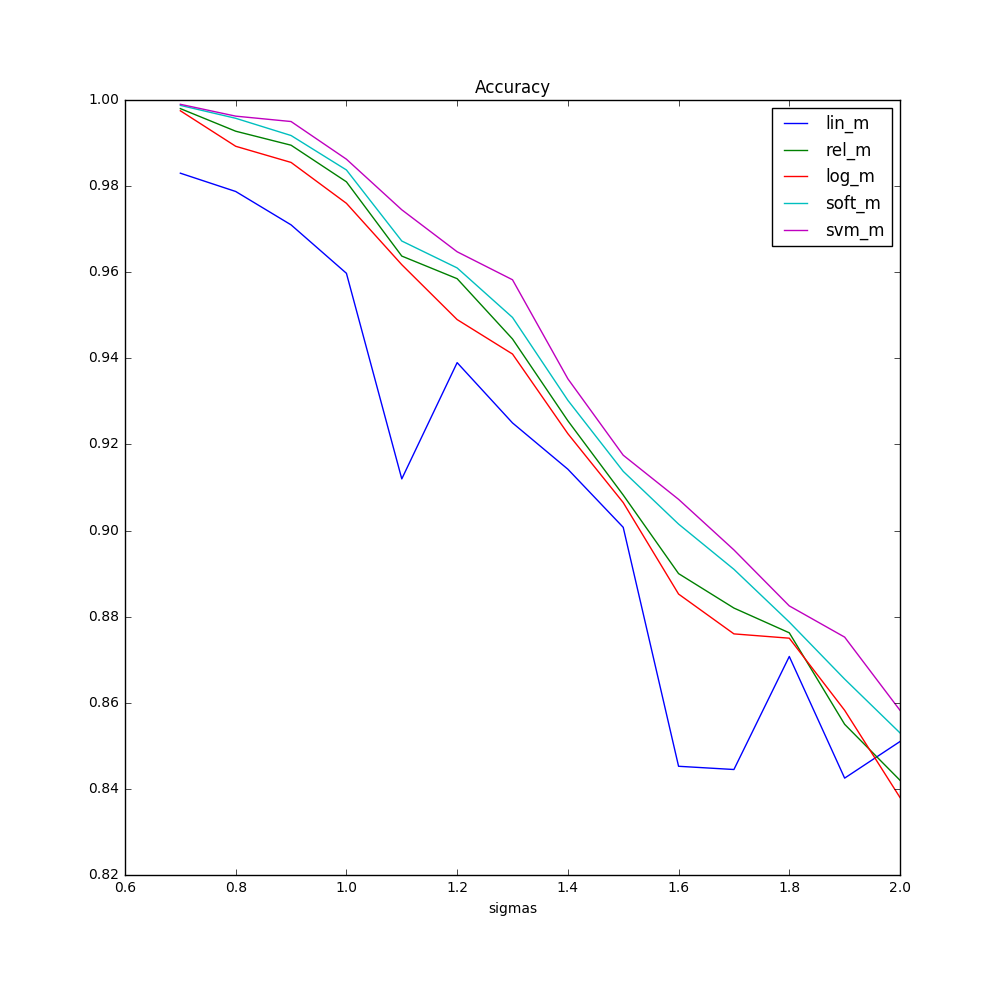
\includegraphics[width=10cm]{first_dataset}
\caption{График доли верных предсказаний для классификатров на 1 выборке}
\label{pic:im1}
\end{figure}

На тестах оказалось, что при увеличении числа признаков довольно сильно начинает проигрывать по веремни работы классификатор, отнованный на решении задачи линейного программирования и логистическая регрессия.

Также его точно сильно флуктуирует. Отбросим его для следующих датасетов с большим числом признаков.

\subsection{Вторая выборка}

Пример генерации выборки:

\begin{lstlisting}
X1 = np.concatenate((np.random.normal(loc=0.5, scale=sigmas[i], size=[int(train_size / 2), 17]),
                    np.random.normal(loc=-0.5, scale=sigmas[i], size=[train_size - int(train_size / 2), 17]))) 
X1 = np.concatenate((X1, np.random.normal(size=[train_size, 3])), axis=1)
y1 = np.concatenate((np.ones(int(train_size / 2)), np.zeros(train_size - int(train_size / 2))), axis=0)
\end{lstlisting}

Тесты были проведены полностью аналогичные первым. В результате сформирован график точностей классификаторов \ref{pic:im2}. Видно, что все классификаторы работают с примерно одинаковой точностью.

\begin{figure}[H]
\centering
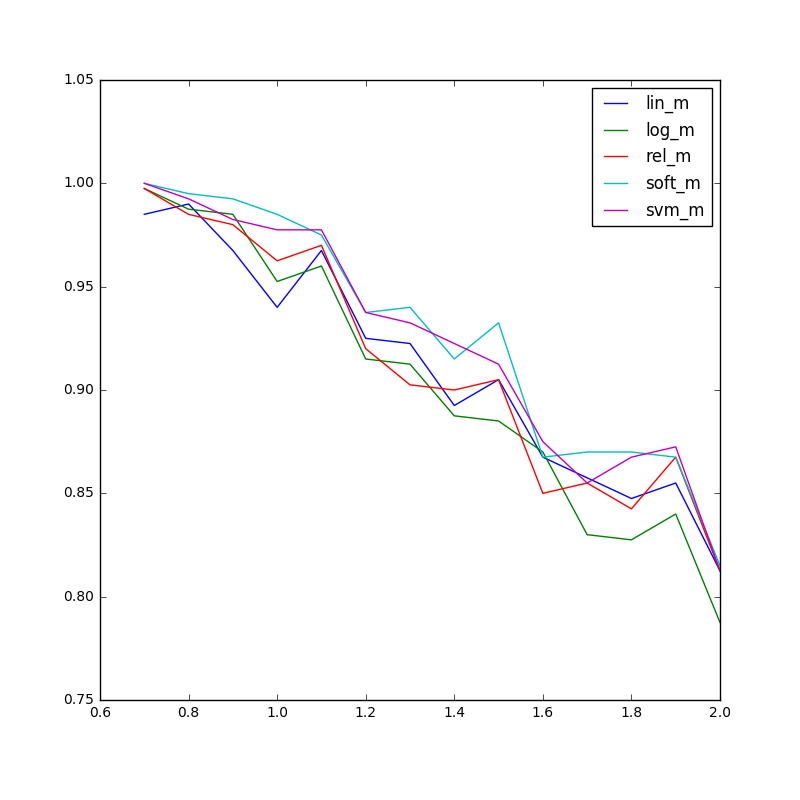
\includegraphics[width=10cm]{second_dataset}
\caption{График доли верных предсказаний для классификатров на 2 выборке}
\label{pic:im2}
\end{figure}

\subsection{Третья выборка}

На данных с такой же дисперсией при большом числе признаков предсказания были верны на всех значениях, поэтому все значения \textbf{sigmas} были увеличены в 10 раз. График с результатами указан на рисунке \ref{pic:im3}.

\begin{figure}[H]
\centering
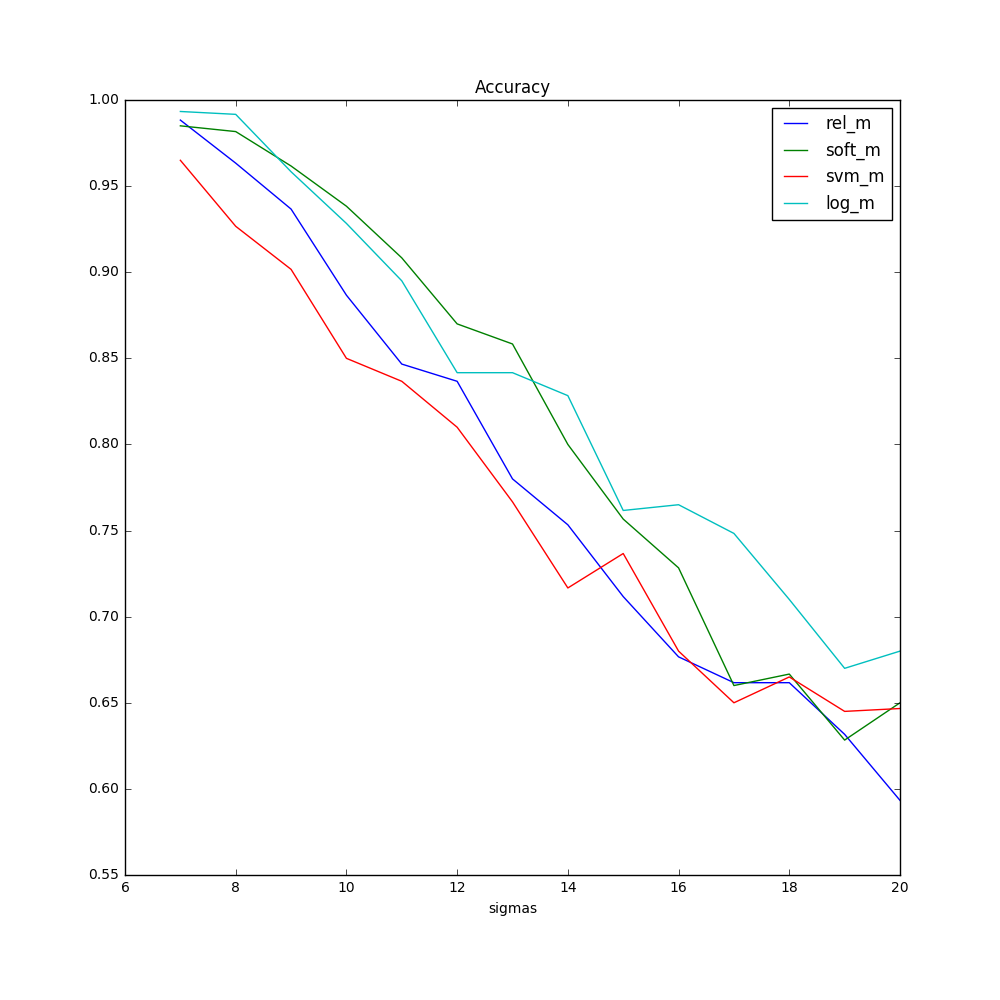
\includegraphics[width=10cm]{third_dataset}
\caption{График доли верных предсказаний для классификатров на 3 выборке}
\label{pic:im3}
\end{figure}


\subsection{Четвёртая выборка}
Датасет содержит 30 признаков, все они числовые, нет нужны в каких-либо преобразованиях, кроме центрирования и деления на стандартное отклонение. Было выбрано 25\% случайных объектов под тетсовую выборку, остальные использовались как обучающая выборка.

Точность предсказаний указана на графике \ref{pic:im5}. Видно, что все классификаторы, кроме первого имеют примерно одинаковые результаты.

\begin{figure}[H]
\centering
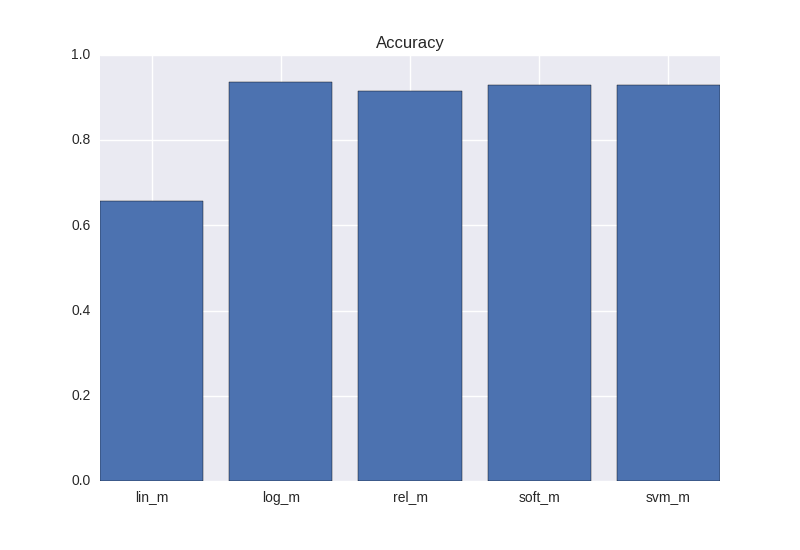
\includegraphics[width=10cm]{fifth_dataset}
\caption{График доли верных предсказаний для классификатров на 4 выборке}
\label{pic:im5}
\end{figure}

\section{Выводы}

\subsection{Реализованы:}
\begin{itemize}
\item Релаксационный метод
\item Метод сведения к линейному программированию
\item Логистическая регрессия
\item Метод опорных векторов
\item Метод минимизации кросс-энтропии
\end{itemize}
\subsection{Исследованы:}
\begin{itemize}
\item качества классификаторов на различных выборках
\item скорости работы на различных выборках
\end{itemize}

\subsection{Проведено сравнение:}

\paragraph{Классификатор, сводящий задачу к линейному программированию}продемонстрировал себя чуть хуже остальных по доле верных предсказаний и был самым медленным. Однако его плюс в том, что если система заранее разделима, то мы сразу получим $\varepsilon \geq 0$, в случае $\varepsilon=0$ нам нужно убедиться, что веса модели не занулились. Неравенство $|\w| > 0$ говорит о том, что есть нормаль к двум полуплоскостям, в которых находятся объекты классов. То есть сведение задачи к линейному программированию позволяет сказать, есть ли между начальными данными разделяющая гиперплоскость.

\paragraph{Логистическая регрессия}, чего и следовало ожидать, проявила себя хорошо и в плане точности предсказаний, и в плане времени работы. 

\paragraph{Релаксадионный метод} также оказался достаточно хорош и работал быстрее остальных. Можно заключить, что он вполне жизнеспособен при условии, что есть уверенность, что и обучающая, и тренировочная выборка достаточно схожи. Основной плюс данного классификатора в высокой скорости работы.

\paragraph{Метод опорных векторов} также проявил себя вполне успешно. Является разумным выбором в случае классификации с большим числом классов, если речь идёт о линейной классификации.

\paragraph{Минимизация кросс-энтропии}, что подтверждается статьями, ведёт себя примерно на одном уровне с методом опорных векторов.

\newpage
\section{Используемая литература}
\begin{thebibliography}{99}
\bibitem{agmon} The relaxation method for linear inequalities, Canad. J. Math. 6(1954), 382-392.
\bibitem{cs231} CS231n Convolutional Neural Networks for Visual Recognition \url{http://cs231n.github.io/linear-classify/}
\end{thebibliography}

\end{document}
